\newcounter{nuserstory}
\newcounter{nusecase}

\newcommand{\userstory}[4]{%
    \refstepcounter{nuserstory}
    \subsection{#1}
    \label{userstory:\thenuserstory}
    \hangindent=40pt
    \textbf{\textit{As a}} #2,\\
    \textbf{\textit{I want to}} #3,\\
    \textbf{\textit{so that}} #4.
}
\newenvironment{usecase}[1]
{
    \refstepcounter{nusecase}%
    \subsection{Use Case \thenusecase: #1}%
    \label{usecase:\thenusecase}%
}{}

% With user stories (\userstory) you can reference them back later with \ref{userstory:n}
% For example, first user story in this file can be referred with \ref{userstory:1}

\chapter{Requirement Analysis}
\label{chap:requirement-analysis}

\section{Stakeholder Analysis}
\label{section:stakeholder-analysis}

\subsection{Primary Stakeholders}
\label{subsection:primary-stakeholders}

\begin{enumerate}[leftmargin=80pt]
    \item \textbf{Users:} The primary stakeholders are the users of our multi-camera tracking system, including security personnel, facility managers, emergency response coordinators, and research analysts.  Their interaction with the system is crucial for effective monitoring, incident response, and data-driven decision-making.  For a detailed specification of our users, see \ref{section:target-user}.
    \item \textbf{System Administrators:}  These individuals are responsible for the installation, configuration, and maintenance of the system.  Their needs include ease of deployment, system stability, and access to diagnostic tools.
    \item \textbf{University/Factory Management:}  These stakeholders are interested in the overall benefits of the system, such as improved safety, optimized resource allocation, and enhanced operational efficiency.  They require reports and data summaries to justify the investment and track performance.
    \item \textbf{MTMMC Dataset Providers/Owners:} The creators and distributors of the Multi-Target Multi-Camera (MTMMC) dataset used for training and evaluating the AI components of this project (\ref{subsection:dataset-information}).
        \begin{itemize}
            \item \textbf{Stake:} They have an interest in ensuring the dataset is used responsibly and ethically, strictly according to the terms and conditions outlined in the usage agreement signed by the project team. This includes preventing misuse or unauthorized redistribution of the data.
            \item \textbf{Project Consideration:} The project must adhere to all stipulations in the dataset usage license. Compliance will be documented, and proper attribution/citation will be provided in all relevant project outputs.
        \end{itemize}
\end{enumerate}

\section{User Stories}
\label{section:user-stories}

%% User Stories Start

\userstory{Continuously Track Individuals Across the Area%
}{security officer%
}{continuously track individuals as they move throughout the monitored area, even when they move between different camera views%
}{I can maintain uninterrupted surveillance of persons of interest and respond quickly to developing situations.}

\userstory{Maintain Tracking During Brief Disappearances%
}{security officer%
}{maintain the track of individuals even if they are temporarily out of sight of all cameras%
}{I can have a complete picture of a person's movements, even if they briefly go around corners or into areas without direct camera coverage.}

\userstory{Visualize Movement Paths%
}{facility manager%
}{see a visual representation of how people move through the facility, including their paths and locations over time%
}{I can understand space usage, identify congestion points, and make informed decisions about facility layout and resource allocation.}

\userstory{Access Historical Movement Data%
}{analytics specialist%
}{access and analyze historical data on individual and group movements, including options to export this data%
}{I can perform in-depth analysis of movement patterns, identify trends, and generate reports to improve operational efficiency and space utilization.  I can also share this data with other systems.}

\userstory{Prioritize Tracking of Specific Individuals%
}{security officer/emergency coordinator%
}{designate specific individuals for increased monitoring and receive immediate updates on their location%
}{I can focus on persons of interest during security incidents or emergencies, ensuring a rapid and effective response.}

\userstory{Ensure System Reliability and Uptime%
}{system administrator%
}{easily monitor system performance, troubleshoot issues, and perform necessary maintenance tasks%
}{I can keep the tracking system running smoothly and minimize disruptions to users.}
%% User Stories End

\section{Use Case Diagram}
\label{section:use-case-diagram}

\begin{figure}[h!]
    \centering
    \begin{tikzpicture}

        % System boundary
        \begin{umlsystem}[x=4]{SpotOn}
            % Use cases inside the system boundary
            \umlusecase[name=track, y=4, width=3cm]{Track Individual Across Cameras}
            \umlusecase[name=maintain, y=1.5, width=4cm]{Maintain Tracking During Temporary Disappearance}
            \umlusecase[name=visualize, y=-1, width=3.5cm]{Visualize Movement Paths on a Map}
            \umlusecase[name=prioritize, y=-3.5, width=4cm]{Prioritize Tracking of Specific Individual}
        \end{umlsystem}

        % Actors outside the system boundary
        \umlactor[x=-4, y=3]{Security Officer}
        \umlactor[x=-4, y=0]{Facility Manager}
        \umlactor[x=-4, y=-2]{Analytics Specialist}
        \umlactor[x=-4, y=-4]{Emergency Coordinator}

        % Associations between actors and use cases
        % Security Officer associations
        \umlassoc{Security Officer}{track}
        \umlassoc{Security Officer}{maintain}
        \umlassoc{Security Officer}{prioritize}

        % Facility Manager association
        \umlassoc{Facility Manager}{visualize}

        % Analytics Specialist association
        \umlassoc{Analytics Specialist}{visualize}

        % Emergency Coordinator association
        \umlassoc{Emergency Coordinator}{prioritize}

    \end{tikzpicture}
    \caption{Use Case Diagram of SpotOn Multi-Camera Tracking System}
    \label{fig:use-case-diagram}
\end{figure}
\clearpage
The use case diagram (Figure \ref{fig:use-case-diagram}) illustrates the interactions between different user roles (actors) and the core functionalities (use cases) of the SpotOn Multi-Camera Tracking System. The actors, shown on the left side of the diagram, represent the primary user groups interacting with the system:

\begin{itemize}
    \item \textbf{Security Officer:} Interacts with tracking, maintaining tracking through gaps, and prioritizing specific individuals.
    \item \textbf{Facility Manager:} Primarily interacts with visualizing movement paths.
    \item \textbf{Analytics Specialist:} Also interacts with visualizing movement paths for analysis.
    \item \textbf{Emergency Coordinator:} Interacts with prioritizing the tracking of specific individuals during critical events.
\end{itemize}
This diagram provides a high-level overview of who uses the system and for what main purposes.

\section{Use Case Model}
\label{section:use-case-model}

\begin{usecase}{Track Individual Across Cameras}
    \textbf{Actors:} Security Officer

    \textbf{Description:} Track an individual's movements across multiple camera views.

    \textbf{Scenario:}
    \begin{enumerate}[leftmargin=80pt]
        \item Log into SpotOn.
        \item Select a location and date.
        \item View available camera feeds.
        \item See people with assigned IDs in each camera view.
        \item View a map showing detected individuals.
        \item Select an individual in any camera view.
        \item See that individual highlighted in all cameras where they appear.
        \item View their movement history on the map.
    \end{enumerate}
\end{usecase}

\begin{usecase}{Maintain Tracking During Temporary Disappearance}
    \textbf{Actors:} Security Officer

    \textbf{Description:} Continue tracking an individual even when temporarily out of camera view.

    \textbf{Scenario:}
    \begin{enumerate}[leftmargin=80pt]
        \item Track an individual in the system.
        \item When the person moves out of all camera views, the system marks this state.
        \item When the person reappears, the system reconnects their identity.
        \item See the individual's complete path, with estimated routes during gaps shown as dashed lines.
    \end{enumerate}
\end{usecase}

\begin{usecase}{Visualize Movement Paths on a Map}
    \textbf{Actors:} Facility Manager/Analytics Specialist

    \textbf{Description:} View movement patterns within a facility for space utilization analysis.

    \textbf{Scenario:}
    \begin{enumerate}[leftmargin=80pt]
        \item Log into SpotOn.
        \item Select a location and date.
        \item View a bird's-eye map of the facility.
        \item See movement paths of all individuals overlaid on the map.
        \item Filter paths by camera view.
        \item Select an individual to highlight only their path.
    \end{enumerate}
\end{usecase}

\begin{usecase}{Prioritize Tracking of Specific Individual}
    \textbf{Actors:} Security Officer/Emergency Coordinator

    \textbf{Description:} Focus system resources on tracking a specific individual.

    \textbf{Scenario:}
    \begin{enumerate}[leftmargin=80pt]
        \item Log into SpotOn.
        \item Select a location and date.
        \item View camera feeds and detected individuals.
        \item Designate an individual for prioritized tracking.
        \item See visual highlighting of the prioritized individual in all cameras.
        \item View their position, detection time, tracking duration, and movement details.
    \end{enumerate}
\end{usecase}

% Use Cases End
% \newpage

\section{User Interface Design}
\label{section:user-interface-design}

The user interface for the multi-camera tracking system is designed to offer a clear, intuitive, and efficient experience for security personnel, facility managers, and other stakeholders, focusing on retrospective analysis of recorded video feeds.  The interface prioritizes the visualization of movement patterns, easy access to detailed tracking information.
% Mockup Start

\begin{figure}[h!]
    \centering
    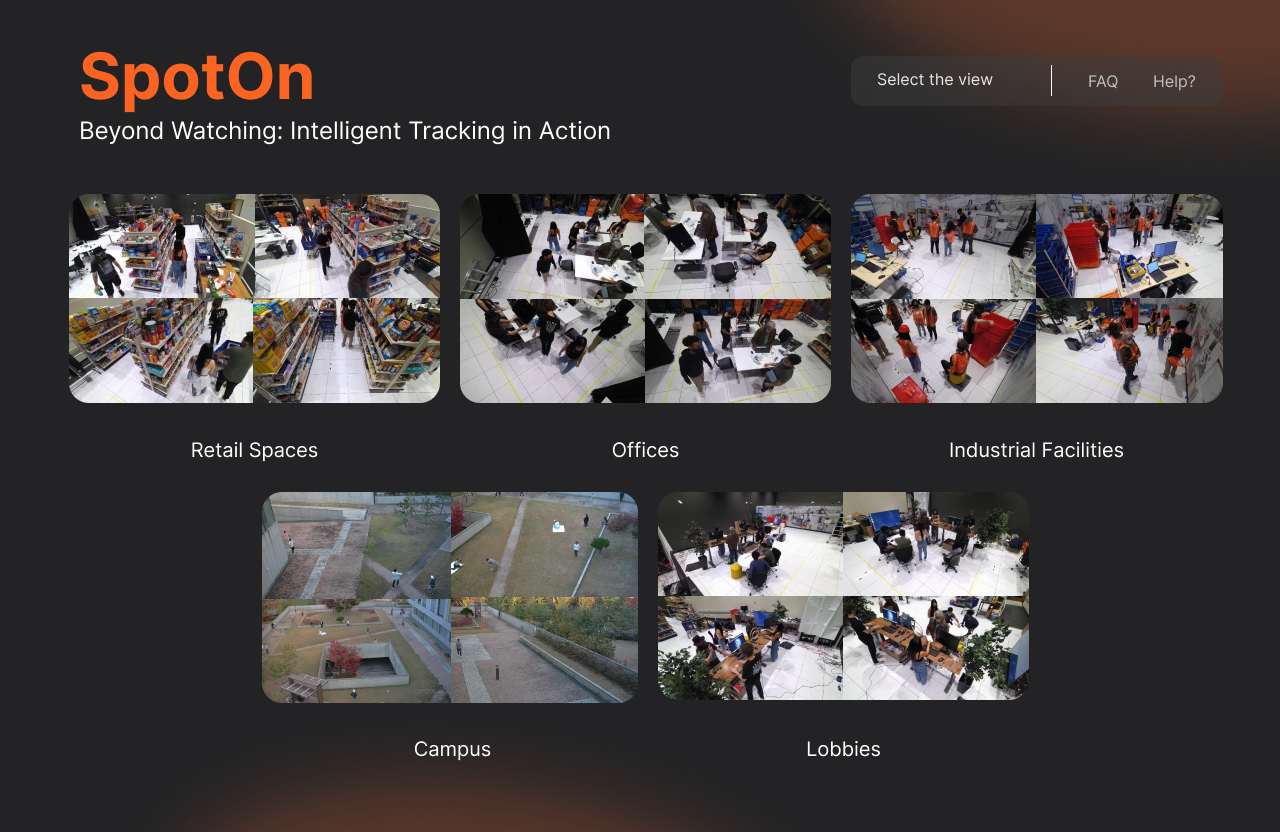
\includegraphics[width=0.8\textwidth,keepaspectratio]{jubjones/mockup/Dashboard.png}
    \caption{Mockup of Landing Page}
    \label{fig:mockup-landing-page}
\end{figure}

\begin{figure}[h!]
    \centering
    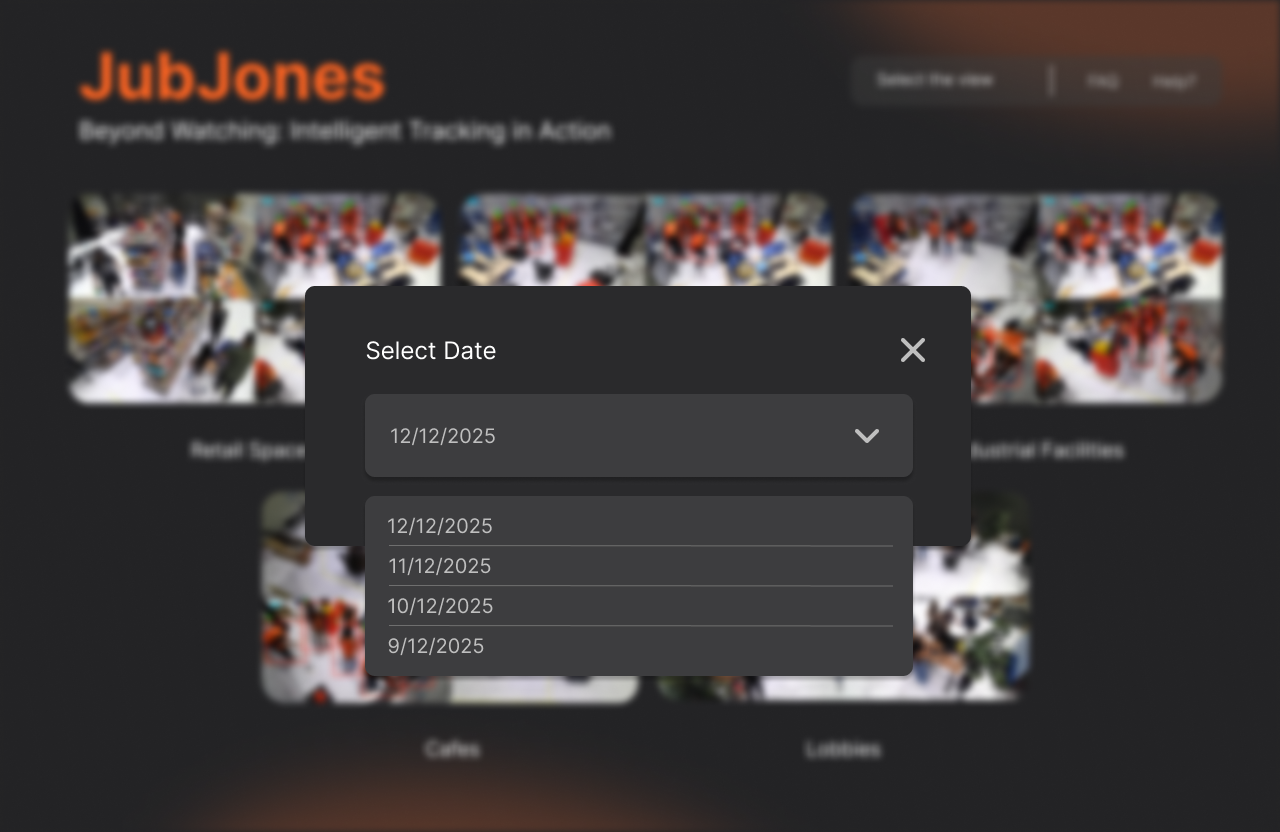
\includegraphics[width=0.8\textwidth,keepaspectratio]{jubjones/mockup/Dashboard - Select toggle.png}
    \caption{Mockup of Landing Page (Date Selection)}
        \label{fig:mockup-landing-page-datetime}
\end{figure}

\begin{figure}[h!]
    \centering
    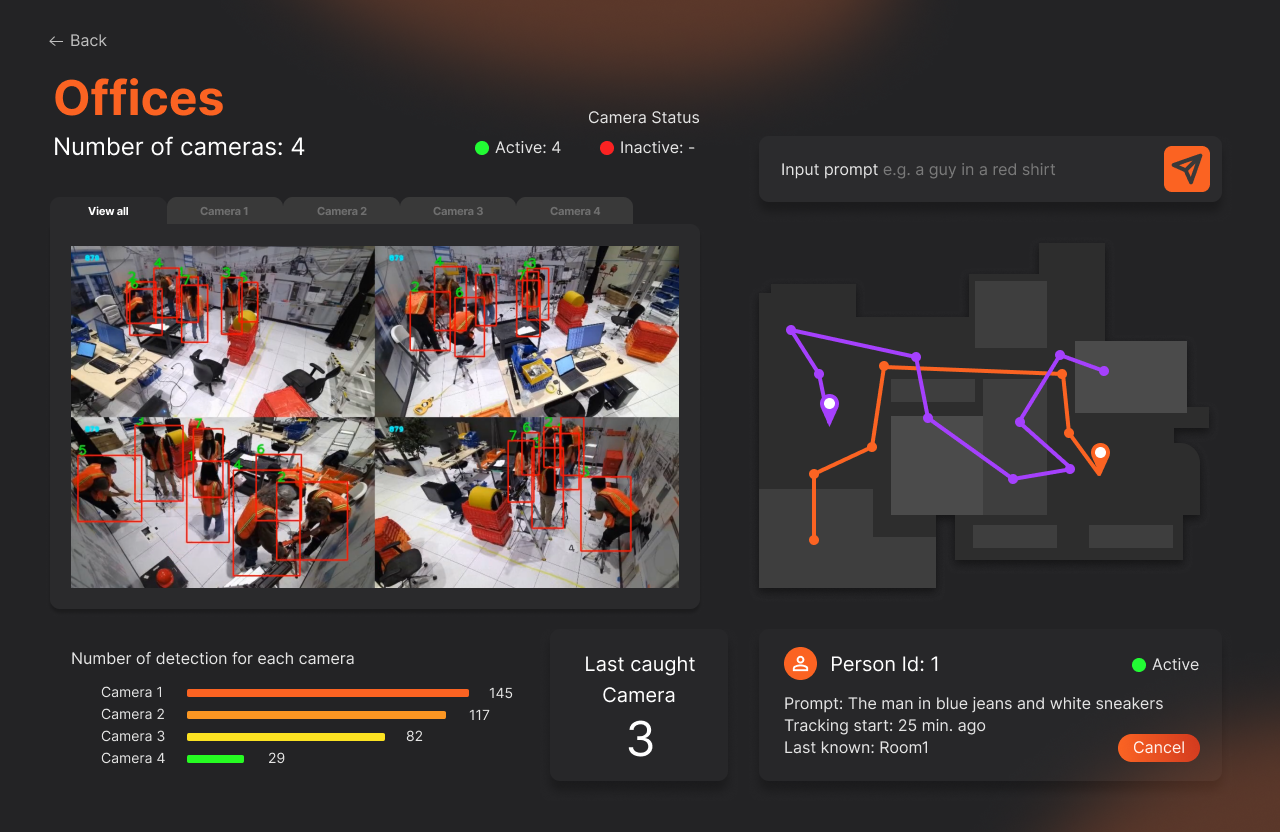
\includegraphics[width=0.8\textwidth,keepaspectratio]{jubjones/mockup/Group view.png}
    \caption{Mockup of Group View Page (Overview)}
    \label{fig:mockup-group-view}
\end{figure}

\begin{figure}[h!]
    \centering
    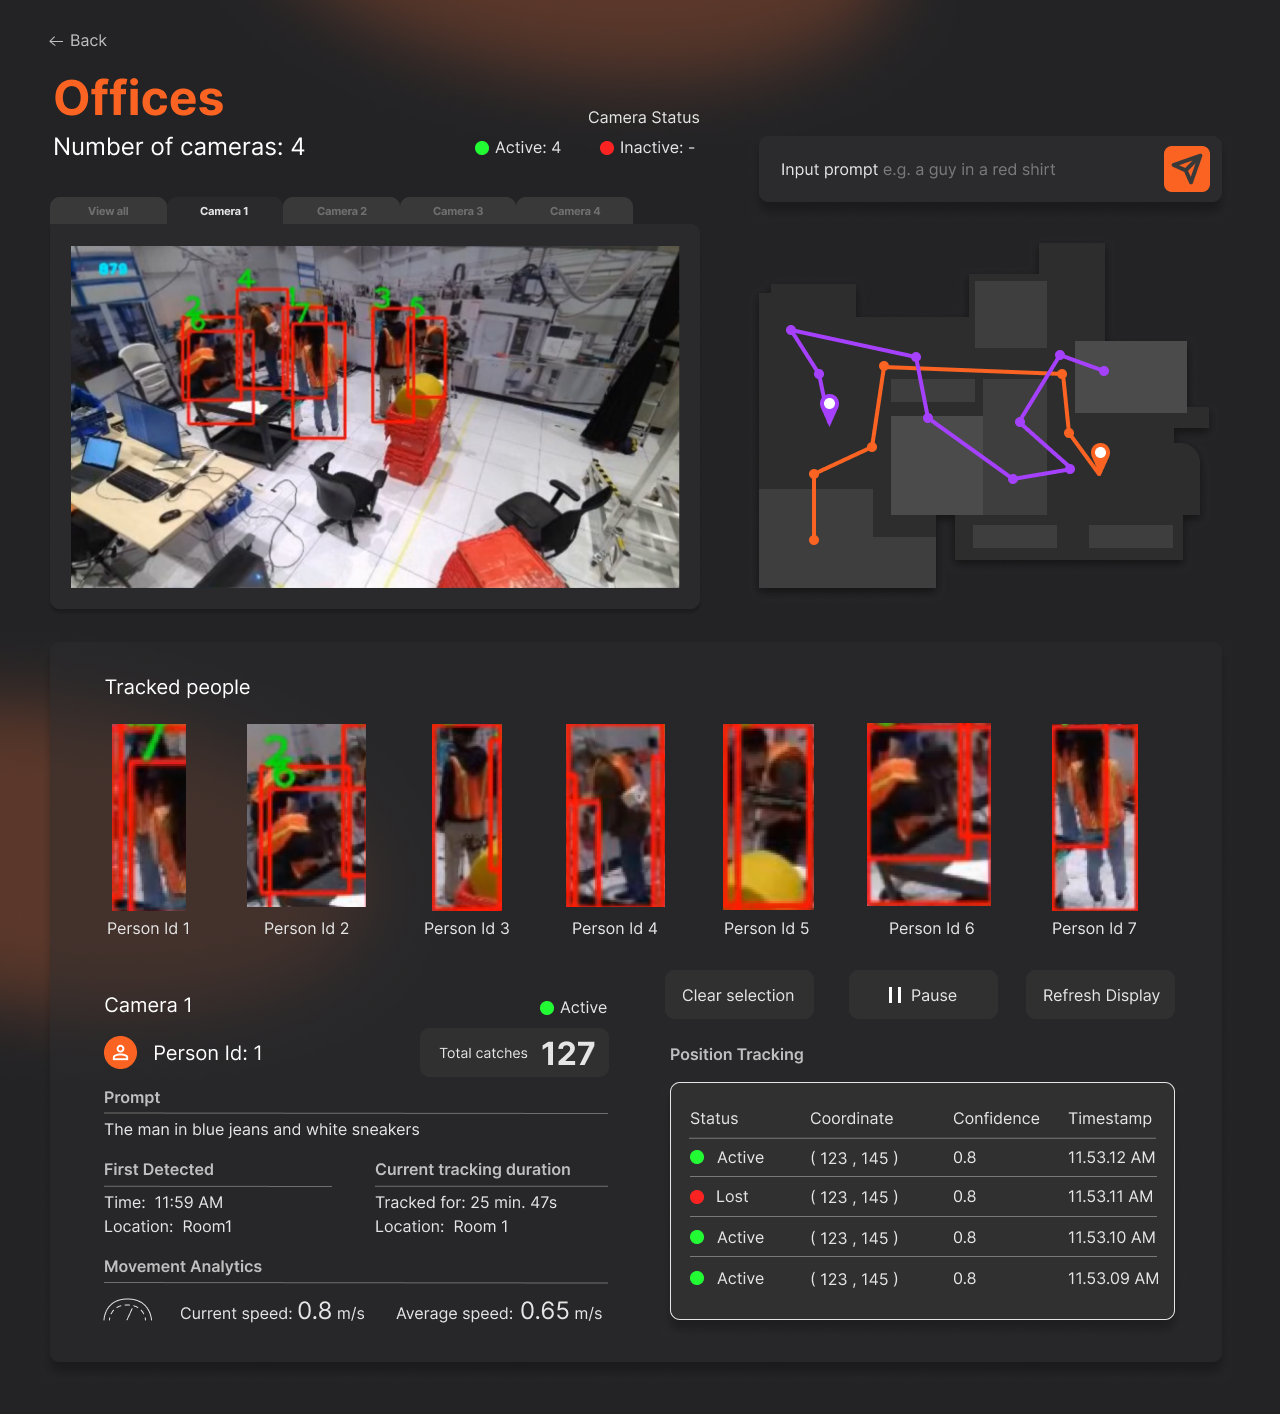
\includegraphics[width=0.8\textwidth, keepaspectratio]{jubjones/mockup/Detail view - expand.png} %Added height constraint
    \caption{Mockup of Group View Page (Expanded - Single Camera View)}
    \label{fig:mockup-group-view-expanded}
\end{figure}
\clearpage

The user interface presents an intuitive flow across multiple views as illustrated in the mockups. The Landing Page (Figure \ref{fig:mockup-landing-page}) offers users a choice between campus and factory views, followed by a date selection interface (Figure \ref{fig:mockup-landing-page-datetime}) to access specific video feed timeframes. Once a selection is made, the Group View Page (Figure \ref{fig:mockup-group-view}) displays all cameras with detected individuals, presenting a comprehensive map that visualizes tracking paths and shows detection counts per camera. This page features multiple tabs, including an overview tab showing all camera feeds simultaneously and individual tabs for specific views. For more detailed analysis, the Expanded Group View (Figure \ref{fig:mockup-group-view-expanded}) displays camera feeds with identification markers for each detected person, listing cropped images of all detected individuals below the video feed. Users can select specific individuals to focus tracking exclusively on them, viewing detailed information such as position tracking status, coordinates, confidence levels, timestamps, first detection time, current tracking duration, and movement analysis.

% Mockup End
\newpage

\section{Target and Development System}
\label{section:development-system}

This section outlines the technical requirements for the development and operation of our multi-camera tracking system, focusing on the capabilities needed to support the user stories and use cases identified earlier.

\subsection{Data Handling and Input Capabilities}
\label{subsection:data-handling-input}
To effectively analyze the multi-camera tracking scenarios, the system must process recorded video data from the MTMMC dataset (\ref{subsection:dataset-information}). Key requirements include:

\begin{itemize}[leftmargin=80pt]
    \item \textbf{Scalable Data Storage Access:} The system must interface with storage solutions capable of holding significant volumes of video data. It requires efficient access mechanisms to retrieve data based on time ranges and camera identifiers, ensuring recorded footage is readily available for retrospective analysis.
    \item \textbf{Historical Data Processing:} The system needs to process recorded video feeds from multiple cameras, potentially spanning different time periods. This capability is essential for batch analysis of past events and movement patterns.
    \item \textbf{Flexible Data Source Configuration:} The system needs a configuration-driven mechanism to specify the location of the input data sources, select specific scenarios or time windows for analysis, and identify the relevant cameras.
\end{itemize}

\subsection{Core Tracking and Analysis Engine Requirements}
\label{subsection:core-tracking-analysis}
The central function of our multi-camera tracking system relies on sophisticated algorithms capable of tracking individuals across multiple camera views. This necessitates several core analytical capabilities:

\begin{itemize}[leftmargin=80pt]
    \item \textbf{Robust Person Detection:} The system requires the ability to accurately detect individuals within diverse single-camera views, handling variations in appearance, lighting, and partial occlusions typical in campus or factory environments (\ref{section:background}).
    \item \textbf{Intra-Camera Tracking Consistency:} Capability to maintain stable tracking of individuals within the field of view of a single camera over consecutive frames, assigning temporary identifiers.
    \item \textbf{Cross-Camera Re-Identification Logic:} A fundamental requirement is the implementation of logic to associate and match individuals across non-overlapping camera views (\ref{section:problem-statement}). This involves comparing extracted appearance features to maintain a persistent identity even with temporal gaps or changes in perspective.
    \item \textbf{Unified Coordinate System Transformation:} The system must be capable of transforming detected locations from individual camera image planes into a common spatial reference frame (e.g., a top-down map). This is essential for visualizing continuous movement paths across the entire monitored environment (\ref{subsection:main-features}).
    \item \textbf{Efficient State and Trajectory Management:} Requires mechanisms for managing the state of numerous tracked individuals (current location, persistent ID, last seen time/camera) and for storing historical trajectory data. This includes both data structures for processing and persistent storage for historical analysis.
\end{itemize}

\subsection{User Interface and Visualization Needs}
\label{subsection:user-interface-visualization}
To deliver actionable insights to users like security officers and facility managers (\ref{section:target-user}), the system must provide an intuitive interface focused on effective visualization of tracking data:

\begin{itemize}[leftmargin=80pt]
    \item \textbf{Multi-Feed Presentation:} The user interface must be designed to display multiple camera feeds concurrently, allowing operators to monitor different areas simultaneously.
    \item \textbf{Integrated Data Overlay:} Requires the capability to overlay tracking information (such as bounding boxes, persistent IDs, status indicators) directly onto the corresponding camera feeds in a clear and understandable manner.
    \item \textbf{Spatial Map Display:} A core requirement is the visualization of movement on a unified map (\ref{subsection:main-features}). The interface must display current positions and historical paths of tracked individuals on this map to provide a comprehensive view of movement patterns.
    \item \textbf{Time-Based Navigation:} Users need the ability to select specific time periods for review and analysis, with controls to navigate through the recorded footage across multiple cameras simultaneously.
    \item \textbf{Responsive Display Framework:} The frontend component must be built using technologies that support efficient rendering of tracking data and provide a clear presentation suitable for monitoring and analysis tasks.
\end{itemize}